\lecture{4}{Суффиксное дерево. Алгоритм Укконена.}
\subsection{Суффиксное дерево}

\begin{definition}
   \highlight{Суффиксное дерево} строки --- бор всех её суффиксов.
\end{definition}

\begin{remark}
    В таком дереве $O(n^2)$ вершин.
\end{remark}

Такое количество вершин нас не устраивает, попробуем его уменьшить.
Заменим все рёбра без ветвления на <<длинные>> рёбра, которые будут представлять собой 
последовательности символов, из которых раньше состояли <<несжатые>> рёбра.
Таким образом, мы получили новые вершины (<<явные>>), 
а также <<неявные>> вершины, которые были у нас в несжатом
дереве, запомним, что они существуют.
Хранить последовательности символов дорого, поэтому будем хранить их как координаты подстроки
в изначальной строке.

\begin{figure}[H]
  \caption*{До <<сжатия>>}
  \begin{center}
    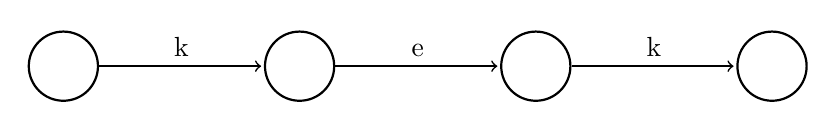
\begin{tikzpicture}[    
      -> = stealth,    
      shorten > = 1pt,    
      auto,    node distance = 3cm,    
      semithick    
      ]    
      
      \tikzstyle{point}=[    
        draw = black,    
        circle,    
        thick,    
        fill = white,    
        minimum size = 25pt    
      ]    
      
      \node[point] (1) [] {};    
      \node[point] (2) [right of=1] {};    
      \node[point] (3) [right of=2] {};    
      \node[point] (4) [right of=3] {};    
      
      \draw (1) -- (2) node[midway, above] {k};
      \draw (2) -- (3) node[midway, above] {e};
      \draw (3) -- (4) node[midway, above] {k};
      
    \end{tikzpicture}
  \end{center}
\end{figure}

\begin{figure}[H]
  \caption*{После}
  \begin{center}
    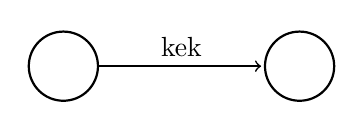
\begin{tikzpicture}[    
      -> = stealth,    
      shorten > = 1pt,    
      auto,    
      node distance = 3cm,    
      semithick    
      ]    
      
      \tikzstyle{point}=[    
        draw = black,    
        circle,    
        thick,    
        fill = white,    
        minimum size = 25pt    
      ]    
      
      \node[point] (1) [] {};    
      \node[point] (2) [right of=1] {};    

      \draw (1) -- (2) node[midway, above] {kek};
      
    \end{tikzpicture}
  \end{center}
\end{figure}

\begin{definition}
  \highlight{Сжатое суффиксное дерево} --- сжатое по описанному выше принципу дерево суффиксов, в каждом
  ребре которого храним координаты подстроки.
\end{definition}

\begin{definition}
  \label{pathway}
  \highlight{Путевая метка} вершины --- координаты подстроки, соответствующей ребру, которое ведёт в вершину. 
\end{definition}


\begin{remark}
  В сжатом суффиксном дереве $O(n)$ вершин.
\end{remark}
Для доказательства достаточно рассмотреть худший случай, когда строка состоит из разных символов.

\begin{remark}
  Пусть в сжатом дереве $n$ листьев, тогда промежуточных вершин $\leq n - 1$.
\end{remark}

\begin{proof}
  Доказательство по индукции. База очевидна, пусть для всех $k \leq n$ выполнено, докажем для $k = n + 1$.

  Рассмотрим корень дерева, пусть его степень равна $2$ (меньше быть не может, т.к. это сжатое
  суффиксное дерево). Пусть в левом поддереве $l_1$ промежуточных вершин,
  а в правом $l_2$, тогда промежуточных вершин из предположения индукции 
  будет $\leq (l_1 - 1) + (l_2 - 1) + 1 = l_1 + l_2 - 1 = l - 1$ (добавляем единицу в конце, т.к. сам корень
  будет промежуточной вершиной.
\end{proof}

Некоторые свойства сжатого суффиксного дерева:
\begin{itemize}
  \item Каждая внутренняя вершина имеет не меньше двух детей.
  \item Каждое ребро помечено непустой подстрокой строки $s$.
  \item Никакие два ребра, выходящие из одной вершины, не могут быть помечены строками, начинающимися с
    одного и того же символа.
  \item Дерево содержит все суффиксы строки, причём каждый суффикс заканчивается точно в листе.
\end{itemize}

Рассмотрим подробнее последний пункт.
На самом деле, сейчас возможна ситуация, когда суффикс заканчивается не в листе, чтобы избежать такого, 
изначально добавим к строке сентилен.

Суффиксные ссылки проводим аналогично, прямо как в боре.
\begin{lemma}
  \label{4.1}
  Для любой внутренней вершины существует суффиксная ссылка, ведущая в некоторую внутреннюю вершину.
\end{lemma}
\begin{proof}
  Рассмотрим некоторую внутреннюю вершину, пусть её путевая метка (\ref{pathway}) 
  равна $s[j\ldots i]$, вершина
  внутренняя, значит в ней есть ветвление, но и вершина, соответствующая путевой метке $s[j + 1\ldots i]$,
  также будет внутренней (ведь ничего не изменится от удаления первого символа ветвление не изменится).
\end{proof}

Теперь попробуем построить сжатое суффиксное дерево. Рассмотрим наивный алгоритм построения
за $O(n^2)$: для каждого символа строки будем добавлять суффикс, начинающийся с него за $O(n)$.

Теперь подробнее рассмотрим процесс добавления отдельного символа в конец строки. 

Возможно несколько случаев:
\begin{enumerate}
  \item Продление листа: пусть у нас суффикс $s[k\ldots i - 1]$ заканчивается в листе, тогда при добавлении
    нового символа $s[i]$ достаточно просто продлить ребро, соответствующее листу. В итоге мы получим, что
    лист останется листом --- это называется  \highlight{инвариантностью листа}. 
   \begin{figure}[H]
     \caption*{До добавления}
     \begin{center}
       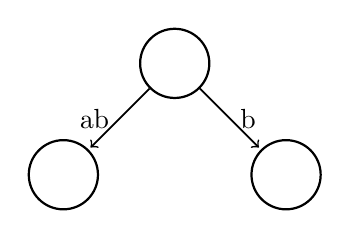
\begin{tikzpicture}[    
         -> = stealth,    
         shorten > = 1pt,    
         auto,    
         node distance = 2cm,    
         semithick    
         ]    
         
         \tikzstyle{point}=[    
           draw = black,    
           circle,    
           thick,    
           fill = white,    
           minimum size = 25pt    
         ]    
         

         \node[point] (1) [] {};    
         \node[point] (2) [below right of=1] {};    
         \node[point] (3) [below left of=1] {};
         
         \draw (1) -- (2) node [midway, right] {b};
         \draw (1) -- (3) node [midway, left] {ab};
         
       \end{tikzpicture}
     \end{center}
   \end{figure}
   \begin{figure}[H]
     \caption*{После}
     \begin{center}
       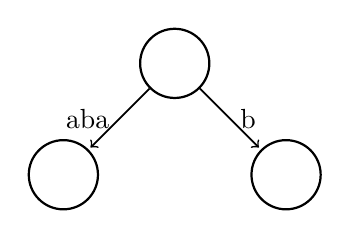
\begin{tikzpicture}[    
         -> = stealth,    
         shorten > = 1pt,    
         auto,    
         node distance = 2cm,    
         semithick    
         ]    
         
         \tikzstyle{point}=[    
           draw = black,    
           circle,    
           thick,    
           fill = white,    
           minimum size = 25pt    
         ]    
         
         \node[point] (1) [] {};    
         \node[point] (2) [below right of=1] {};    
         \node[point] (3) [below left of=1] {};    

         \draw (1) -- (2) node [midway, right] {b};
         \draw (1) -- (3) node [midway, left] {aba};
         
       \end{tikzpicture}
     \end{center}
   \end{figure}

  \item Ответвление. Пусть при добавлении нового символа $c$ 
    мы пришли в вершину (явную или неявную), но не лист.
    \begin{itemize}
      \item Тогда если мы пришли в явную вершину, то нам достаточно добавить лист и соединить этот лист с 
            нашей явной вершиной ребром, соответствующим символу $c$.
      \begin{figure}[H]
        \caption*{До добавления}
        \begin{center}
          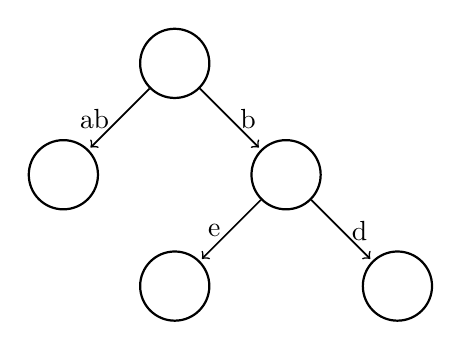
\begin{tikzpicture}[    
            -> = stealth,    
            shorten > = 1pt,    
            auto,    
            node distance = 2cm,    
            semithick    
            ]    
            
            \tikzstyle{point}=[    
              draw = black,    
              circle,    
              thick,    
              fill = white,    
              minimum size = 25pt    
            ]    
            

            \node[point] (1) [] {};    
            \node[point] (2) [below right of=1] {};    
            \node[point] (3) [below left of=1] {};
            \node[point] (4) [below left of=2] {};
            \node[point] (5) [below right of=2] {};
            
            \draw (1) -- (2) node [midway, right] {b};
            \draw (1) -- (3) node [midway, left] {ab};
            \draw (2) -- (4) node [midway, left] {e};
            \draw (2) -- (5) node [midway, right] {d};
            
          \end{tikzpicture}
        \end{center}
      \end{figure}
      \begin{figure}[H]
        \caption*{После}
        \begin{center}
          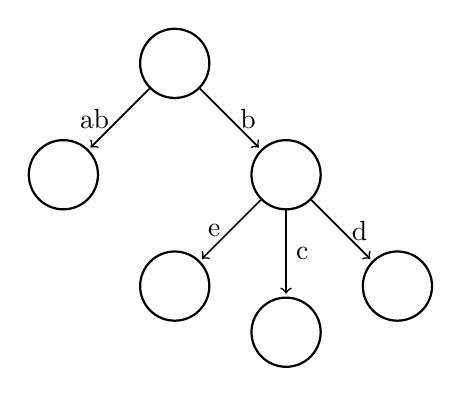
\begin{tikzpicture}[    
            -> = stealth,    
            shorten > = 1pt,    
            auto,    
            node distance = 2cm,    
            semithick    
            ]    
            
            \tikzstyle{point}=[    
              draw = black,    
              circle,    
              thick,    
              fill = white,    
              minimum size = 25pt    
            ]    
            
            \node[point] (1) [] {};    
            \node[point] (2) [below right of=1] {};    
            \node[point] (3) [below left of=1] {};
            \node[point] (4) [below left of=2] {};
            \node[point] (5) [below right of=2] {};
            \node[point] (6) [below of=2] {};
            
            \draw (1) -- (2) node [midway, right] {b};
            \draw (1) -- (3) node [midway, left] {ab};
            \draw (2) -- (4) node [midway, left] {e};
            \draw (2) -- (5) node [midway, right] {d};
            \draw (2) -- (6) node [midway, right] {c};
            
          \end{tikzpicture}
        \end{center}
      \end{figure}
      \item Если же мы пришли в неявную вершину, то необходимо сделать эту вершину явной (т.к. от неё
            появляется ветвление), добавить новый лист, в который ведёт ребро символа $c$, и
            соединить с этой вершиной.

      \begin{figure}[H]
        \caption*{До добавления}
        \begin{center}
          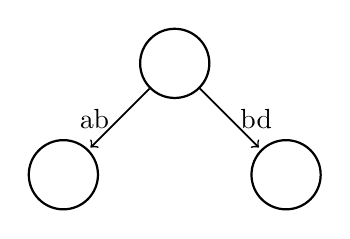
\begin{tikzpicture}[    
            -> = stealth,    
            shorten > = 1pt,    
            auto,    
            node distance = 2cm,    
            semithick    
            ]    
            
            \tikzstyle{point}=[    
              draw = black,    
              circle,    
              thick,    
              fill = white,    
              minimum size = 25pt    
            ]    
            

            \node[point] (1) [] {};    
            \node[point] (2) [below right of=1] {};    
            \node[point] (3) [below left of=1] {};
            
            \draw (1) -- (2) node [midway, right] {bd};
            \draw (1) -- (3) node [midway, left] {ab};
            
          \end{tikzpicture}
        \end{center}
      \end{figure}
      \begin{figure}[H]
        \caption*{После}
        \begin{center}
          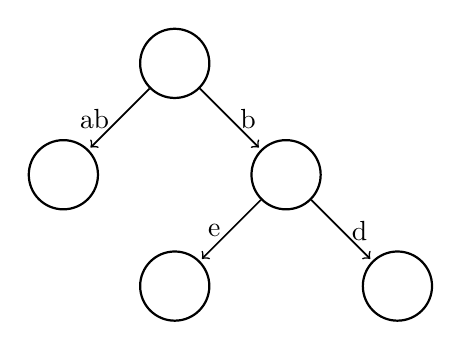
\begin{tikzpicture}[    
            -> = stealth,    
            shorten > = 1pt,    
            auto,    
            node distance = 2cm,    
            semithick    
            ]    
            
            \tikzstyle{point}=[    
              draw = black,    
              circle,    
              thick,    
              fill = white,    
              minimum size = 25pt    
            ]    
            
            \node[point] (1) [] {};    
            \node[point] (2) [below right of=1] {};    
            \node[point] (3) [below left of=1] {};
            \node[point] (4) [below right of=2] {};
            \node[point] (5) [below left of=2] {};
            
            \draw (1) -- (2) node [midway, right] {b};
            \draw (1) -- (3) node [midway, left] {ab};
            \draw (2) -- (4) node [midway, right] {d};
            \draw (2) -- (5) node [midway, left] {e};
            
          \end{tikzpicture}
        \end{center}
      \end{figure}
    \end{itemize}
  \item Ничего не делать. Такая ситуация возникает, если из суффикса, по которому мы идём, если путь
        по нашему символу.
\end{enumerate}

Запомним эти переходы и их номера.

\subsection{Алгоритм Укконена.}
Теперь перейдём ближе к алгоритму. Как говорилось ранее, шаг алгоритма подразумевает
добавление символа к каждому суффиксу. Мы уже говорили выше, какие типы добавления бывают.
Заметим, что с помощью суффиксных ссылок мы можем легко перейти к суффиксу с длиной меньше на 1.
Таким образом, нам достаточно переходить по суффиксным ссылкам до корня и постепенно добавлять
к суффиксам наш новый символ.

Заметим, что на очередном шаге типы позиций (3 типа, которые описаны выше) могут изменяться определённым образом, а именно:
\begin{itemize}
  \item $1 \to 1 \colon$, т.е. лист остаётся листом (про это мы уже разговаривали)
  \item $2 \to  1$, на картинках видно, что мы всегда добавляем лист
  \item $3 \to  3, 2$, т.к. переход приведёт к позиции, из которой либо есть переход по следующему символу, либо нет, но там точно не лист
\end{itemize}

Теперь докажем важную лемму, которая позволит окончательно сформулировать алгоритм.
\begin{lemma}
  Пусть мы находимся на фазе добавления нового символа в некоторый $j$-ый суффикс. Тогда если мы встретили
  тип добавления $3$, все следующие добавления к меньшим суффиксам будет этого же типа. Т.е. мы можем
  остановить вставку, как только мы встретили тип вставки $3$.
\end{lemma}
\begin{proof}
  Если путь с меткой $s[j\ldots i - 1]$ с типом вставки $3$ продолжается символом $i$, то и путь 
  $s[j + 1\ldots i - 1]$ будет продолжаться этим же символом $i$.
\end{proof}

Осталось избавиться от обработки типа $1$, действительно, при вставке элемента тип не поменяется, тогда
<<продлим>> листья изначально до бесконечности, что позволит не продлевать на $1$ на каждом шаге.

Итоговый алгоритм:
\begin{itemize}
  \item Обрабатываем один символ
  \item Вершины типа $1$ изначально все продлили до бесконечности
  \item Обрабатываем вершины типа $2$ 
  \item Как только обработали вершину типа $3$, заканчиваем шаг, запоминаем индекс
  \item На следующем шаге начинаем обработку с этого индекса, т.к. все вершины до него стали типа $1$ или уже
    были этого типа
\end{itemize}

Осталось только научиться считать суффиксные ссылки, будем это делать аналогично Ахо-Корасику: поднимемся 
до ближайшей явной вершины, перейдём по её суффиксной ссылке (она существует по \ref{4.1}) и продлим её 
нашим исходным символом. (спуск после перехода по суффиксной ссылке можно делать не сравнивая все символы
ребра, а только первый символ и длину подстрок, это возможно, т.к. суффиксная ссылка приведёт к суффиксу
изначальной ветки, а значит там точно будет путь по этим символам).

\begin{figure}[H]
  \caption*{Пример}
  \begin{center}
    \begin{tikzpicture}[    
      -> = stealth,    
      shorten > = 1pt,    
      auto,    
      node distance = 3cm,    
      semithick    
      ]    
      
      \tikzstyle{point}=[    
        draw = black,    
        circle,    
        thick,    
        fill = white,    
        minimum size = 25pt    
      ]    
      
      \node[point] (1) [] {$s_{r}$};    
      \node[point] (2) [right of=1] {$s_{r}$};    
      \node[point] (3) [below right of=2] {$s_{i}$};    
      \node[point] (4) [below left of=1] {$s_{i - 1}$};    
      
      \draw (2) -- (1) node [midway, above] {переход} node [midway, below] {по ссылке}; 
      \draw (3) -- (2) node [midway, right] {возврат по ребру}; 
      \draw (1) -- (4) node [midway, left] {спуск по вершинам}; 

    \end{tikzpicture}
  \end{center}
\end{figure}
В примере нам нужно посчитать суффиксную ссылку для $s_{i}$, мы переходим в ближайшую явную вершину
$s_{r}$, переходим по её суффиксной ссылке, а дальше спускаемся по тем же вершинам (какие содержаться в
ребре, по которому мы поднялись).

\subsection{Доказательство асимптотики.}
Для начала рассмотрим вспомогательные понятия:
\begin{definition}
  \highlight{Глубина вершины} --- число рёбер на пути от корня до вершины.
\end{definition}

\begin{lemma}
  \label{4.3}
  При переходе по суффиксной ссылке глубина уменьшается не более чем на $1$. 
\end{lemma}
\begin{proof}
  Прямо следует из определения суффиксной ссылки. Пусть путь из корня в исходную вершину 
  $A = s[j + 1\ldots i]$, а путь в вершину, куда мы приходим по суффиксной ссылке $B = s[j\ldots i]$.
  Они будут различаться на $1$ только в случае, когда в первую вершину на пути $B$ ведёт
  ребро из одного символа.
\end{proof}

\begin{lemma}
  \label{4.4}
  Число переходов по рёбрам внутри фазы (вставка текущего символа) номер $i$ равно $O(i)$.
\end{lemma}
\begin{proof}
  Найдём количество переходов по рёбрам при поиске конца суффикса. Переход во внутреннюю вершину 
  уменьшает глубину на $1$, переход по суффиксной ссылке уменьшает глубину не более чем на $1$. (\ref{4.3})
  Таким образом, мы уменьшаем глубину не более чем на $2$.
  Так как высота не может увеличиться больше глубины дерева, то суммарно высота не может увеличиться больше,
  чем на $2i$. Получаем число переходов по рёбрам за одну фазу $O(i)$.
\end{proof}

\begin{theorem}[Асимптотика алгоритма Укконена]
  Алгоритм Укконена работает за $O(n)$.
\end{theorem}
\begin{proof}
  В течение работы алгоритма создаётся не более $O(n)$ вершин (действительно, если у нас у каждой вершины
  хотя бы два ребёнка, а число листов по определению $n$, то из индукции по  $n$ легко следует 
  это утверждение, основная идея в том, чтобы отрезать листья и сводить к предположению индукции). 
  Все суффиксы, который заканчиваются в листах (тип $1$) мы продлеваем за $O(1)$, случаи типа  $3$ 
  мы вовсе не обрабатываем, а за обработку случаев $2$ суммарно будет создано не более $O(n)$ вершин 
  (так как их всего $O(n))$, т.е. амортизационно на каждой фазе будет создано  $O(1)$ вершин.
  Каждую фазу мы начинаем добавление суффикса не с корня, а с индекса, на котором в предыдущей фазе
  было применено правило $3$, то суммарное количество переходов (из \ref{4.4}) будет $O(n)$ или  $O(1)$
  амортизационно. 
\end{proof}

